% ------------------------------------------------------------------------ %
% !TEX encoding = UTF-8 Unicode
% !TEX TS-program = pdflatex
% !TEX root = ../Tesi.tex
% !TEX spellcheck = it-IT
% ------------------------------------------------------------------------ %
%
% ------------------------------------------------------------------------ %
% 	NOME CAPITOLO
% ------------------------------------------------------------------------ %
%
\chapter{Software Ethereum-based per Blockchain private: Quorum}
%
\label{cap:quorum}
%
% ------------------------------------------------------------------------ %
%
\section{Introduzione}
%
Come abbiamo scritto nei precedenti capitoli, gli Smart Contract si presentano come un libro mastro condiviso e replicato in ambiente Enterprise con la promessa di migliorare l'efficienza e diminuire i costi comparati con le altre soluzioni fornite da sistemi enterprise pre-esistenti\footnote{Ad esempio Zcash} basati sulla logica di business duplicata e su un protocollo del consenso basato sulla riconciliazione. Però gli attuali sistemi basati su smart contracts non sono capaci di fornire la privacy di dati essendo lo stato delle transazioni e degli smart contract esposti in chiaro nella rete. Questo lavoro di tesi concentra la sua attenzione su una blockchain che è stata costruita sulle specifiche di Ethereum e poi modificata per ottenere i requisiti di privatezza in ambiente enterprise, dove avviene lo scambio dati sensibili (come ad esempio i dati medici).\\
\emph{Quorum}\autocite{website:quorum} è un libro mastro distributo, privato, permissioned ed Ethereum-based che è stato sviluppato da J.P. Morgan per fornire all'industria dei servizi finanziari un'implementazione di Ethereum basata su permessi che possa supportare la privacy di contratti e transazioni. Quorum include quindi un fork minimo del client Ethereum (ovvero geth) facendo così leva sui traguardi tecnologici raggiunti dalla comunità degli sviluppatori di Ethereum.\footnote{ La libreria go-ethereum e i suoi file binari sono licenziati sotto la GNU Lesser General Public License v3.0} Le feature principali di Quorum, che corrispondono anche alle principali aggiunte rispetto alla blockchain pubblica Ethereum, sono:
\begin{enumerate}
	\item privatezza di contratti e transazioni. Quorum supporta transazioni e contratti privati attraverso la separazione tra stato pubblico e privato servendosi di \emph{constellation} uno strumento per lo scambio di messaggi criptati peer-to-peer per lo scambio diretto privati tra i partecipanti della rete;
	\item meccanismo di consenso basato sul voto multiplo. Essendo quorum una blockchain privata i partecipanti sono noti e non è strettamente necessario utilizzare la proof-of-work;
	\item gestione dei permessi sia a livello di rete che a livello di singolo peer. Il permissioning viene realizzato utilizzando la logica degli smart contracts;
	\item performance maggiori rispetto alla sua controparte pubblica.
\end{enumerate}%
%
\begin{figure}[H]
	%
	\centering
	%
	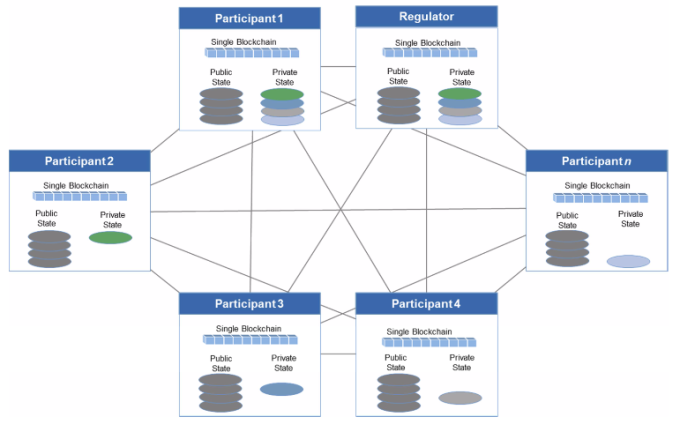
\includegraphics[width=.9\textwidth]{Quorum/quorum}
	%
	\caption{Diagramma di Quorum}
	%
	\label{fig:diagramma di quorum}
	%
\end{figure}
%
Lo scopo principale degli sviluppatori è stato quello di riutilizzare per quanto possibile l'attuale tecnologia minimizzando i cambiamenti rispetto all'attuale versione di Ethereum sia per favorire i tempi di sviluppo e deploy delle applicazioni decentralizzate sia per minimizzare lo sforzo di mantenere sincronizzata la code-base comune di Ethereum presente in Quorum. Inoltre, anche se è stata pensata in prima istanza per implementare servizi finanziari in cui si vuole comunque mantenere una figura di tipo controllore all'interno della rete, è possibile utilizzare Quorum per ambiti esterni alla finanza in quanto mantiene tutte l'espressività a livello di codice della blockchain Ethereum.
%
\section{Architettura}
%
Attualmente Quorum include le seguenti componenti:
%
\begin{figure}[H]
	%
	\centering
	%
	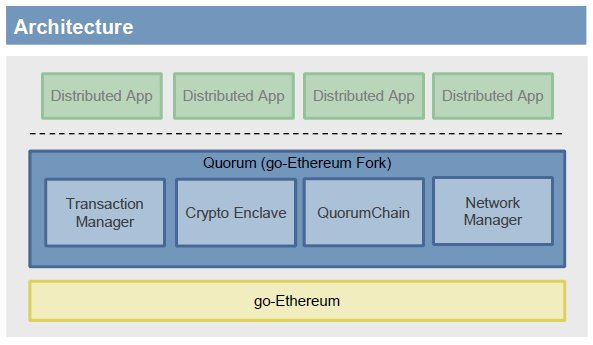
\includegraphics[width=.9\textwidth]{Quorum/comp}
	%
	\caption{Componenti di Quorum}
	%
	\label{fig:componenti di quorum}
	%
\end{figure}
%
L'essenza di Quorum è quella di utilizzare la crittografia al fine di prevenire l'accesso ai dati sensibili a chiunque, eccetto per gli utenti coinvolti. Questa soluzione è stata realizzata utilizzando una singola blockchain condivisa e combinando l'architettura software degli smart contract (che fornisce la segmentazione dei dati privati) e le modifiche al client Ethereum (che include le modifiche al processo di proposta e validazione dei blocchi). Le sue componenti principali sono le seguenti:
%
\paragraph{Quorum Node}
%
Un nodo Quorum corrisponde al client geth modificato. Rispetto alla sua controparte pubblica contiene le seguenti modifiche:
\begin{enumerate}
	\item l'algoritmo di consenso basato sulla proof-of-work è stato rimpiazzato da un meccanismo di tipo vote-based (più adatto alle blockchain private) denominato \emph{QuorumChain}. Quorum attualmente offre anche delle alternative rispetto a QuorumChain stesso:
	      \begin{itemize}
	      	\item \emph{Raft-based Consensus}: un modello di consenso per tempi di blocco maggiori, immutabilità delle transazioni e creazioni di blocchi on-demand.
	      	\item \emph{Istanbul BFT}: un algoritmo di consenso basato sul "Practical Byzantine Fault Tolerance" (PBFT).\cite{pbft}
	      \end{itemize}%
	\item il layer P2P è stato modificato al fine di permettere connessioni solo da/verso nodi autorizzati;
	\item sia la logica di generazione del blocco che la logica di validazione del blocco sono state modificate per sostituire il "Global state root" nel block header di Ethereum con il "Global public state root". Inoltre la logica di validazione del blocco è stata ulteriormente modificata per supportare le transazioni private;
	\item il Patricia tree è stato diviso in: public state tree e private state tree;
	\item la creazione delle transazioni è stata modificata per permettere che i dati della transazione vengano sostituiti con l'hash crittografico al fine di preservare la privatezza del dato quando richiesto;
	\item Il prezzo del Gas è stato rimosso (anche se il concetto di gas rimane presente all'interno della blockchain).
\end{enumerate}%
%
\paragraph{Constellation}
%
Constellation è un sistema general purpose per trasmettere informazioni in modo sicuro. Può essere paragonato ad una rete di MTA (Message Transfer Agents) dove i messaggi sono criptati tramite il software \enquote*{\gls{pgp}}. Non è un modulo pensato specificatamente per le blockchain ma è utilizzabile ogni volta che si vuole scambiare messaggi \enquote*{sigillati} individualmente all'interno di una rete di partecipanti. Questo componente è composto da due sotto componenti: il nodo Constellation (che viene utilizzato nell'implementazione standard del \emph{PrivateTransactionManager}) ed Enclave.%
\subparagraph{Il Transaction Manager.} È responsabile per la privacy delle transazioni. Esso infatti conserva e permette l'accesso ai dati criptati delle transazioni, lo scambio di payload criptati con i transaction manager degli altri partecipanti e, al tempo stesso, non ha accesso ad alcuna chiave privata sensibile. Utilizza Enclave per le funzionalità crittografiche. Ogni Quorum node possiede il suo Transaction Manager che dialoga con le sue controparti distribuite sugli altri nodi.%
\subparagraph{Enclave.} Abbiamo visto come i protocolli di ledger distribuiti facciano tipicamente uso di tecniche crittografiche per l'autenticità delle transazioni, l'autenticazione dei partecipanti e la conservazione storica dei dati (attraverso una catena di hash crittografici dei dati). Al fine di ottenere una separazione di compiti e al tempo stesso di garantire un miglioramento delle performanze attraverso la parallelizzazione delle operazioni che riguardano la crittografia, la maggior parte del lavoro crittografico inclusa la generazione di chiavi simmetriche e la cifratura/decifratura dei dati è delegata appunto ad Enclave. \\ Questo componente lavora quindi insieme al transaction manager per rafforzare la privacy attraverso la gestione della cifratura/decifratura in modo isolato. Esso quindi si comporta a tutti gli effetti come un \enquote*{Hardware Security Module} (HSM) isolato da tutti gli altri componenti.
%
\paragraph{Il Network Manager} si occupa del controllo degli accessi alla rete, permettendo quindi la creazione di una rete permissioned. %
%
\section{Transazioni}
%
Un'altra delle feature chiave di Quorum, come abbiamo detto, è la privatezza delle transazioni. Quorum infatti introduce la nozione di \emph{transazione privata} contrapposta alla classica \emph{transazione pubblica}. Questo però non vuol dire che gli sviluppatori di quorum hanno introdotto un nuovo tipo di transazione stravolgendo quindi il modello di Ethereum, bensì hanno esteso l'Ethereum Transaction Model nel seguente modo:
\begin{itemize}
	\item viene aggiunto un parametro opzione \emph{privateFor}\footnote{privateFor è un array di chiavi pubbliche} che, quando specificato, contraddistingue una transazione come privata e i nodi della blockchain la tratteranno di conseguenza;
	\item viene aggiunto un nuovo metodo al Transaction Type, denominato \emph{isPrivate}, necessario per identificare le nuove transazioni private.
\end{itemize}%
\paragraph{Transazioni pubbliche}%
Le transazioni pubbliche sono quelle transazioni in cui il payload è visibile a tutti i partecipanti della rete Quorum (hanno la stessa visibilità delle transazioni in Ethereum). Questo tipo di transazione viene eseguito nel modo standard di Ethereum ovvero se una transazione pubblica viene inviata ad un account che possiede il codice di un contratto, ogni partecipante eseguirà lo stesso codice e il loro stateDb verrà aggiornato di conseguenza. Il valore $V$ della firma della transazione viene settato dal nodo Quorum a $27 o 28$.
%
\paragraph{Transazioni private}%
Le transazioni private sono quelle transazioni in cui il payload è visibile solamente ai partecipanti della rete le cui chiavi pubbliche sono specificate nel parametro privateFor della transazione. Quando il nodo di Quorum incontra una transazione con un parametro privateFor non nullo, setta il valore $V$ della firma della transazione a $37 o 38$. Le transazioni private non sono eseguite nella modalità standard di Ethereum. Infatti prima che il nodo di Quorum del mittente propaghi la transazione al resto della rete, rimpiazza il payload originale della transazione con un hash del payload crittografato che riceve dal modulo Constellation. I partecipanti che fanno parte della transazione potranno rimpiazzare l'hash con il payload attuale attraverso la loro istanza di Constellation, chiamare l'EVM per l'esecuzione ed il loro stateDb sarà aggiornato di conseguenza. Invece i partecipanti che non fanno parte della transazione potranno leggere solamente l'hash e non eseguiranno la transazione (la transazione sarà a tutti gli effetti saltata da loro). Quindi questi due set di partecipanti termineranno con differenti stateDb e non potranno raggiungere il consenso perciò Quorum, al fine di supportare questa "biforcazione" dello stato del contratto immagazzina lo stato del contratto pubblico in un \emph{Public State trie} sincronizzato globalmente mentre immagazzina lo stato dei contratti privati in un \emph{Private state trie} non sincronizzato globalmente. Inoltre un contratto privato può essere creato solo attraverso una transazione privata.\\
Per una descrizione del flusso di una transazione privata all'interno di Quorum, si rimanda all'\autoref{cap:transaction}.%
\section{Consenso in Quorum}
%
Quorum\footnote{Nella sua versione studiata 1.5} supporta il meccanismo di consenso denominato \emph{QuorumChain}, un algoritmo a tempo a maggioranza di voto che utilizza:
\begin{enumerate}
	\item uno smart contract per governare il consenso e gestire chi può partecipare al consenso;
	\item transazioni Ethereum per propagare i voti attraverso la rete;
	\item validazione della firma di Ethereum per validare le firme ricevute dai nodi \emph{maker} e \emph{voter}.
\end{enumerate}%
Quorum utilizza nel meccanismo di consenso una divisione di ruoli tra i nodi. Infatti all'interno della rete possono esistere nodi con il ruolo di \emph{Voter} il quale permette loro di votare quale blocco dovrebbe essere la testa canonica ad una particolare altezza. Il blocco più recente con la maggioranza dei voti viene considerato la testa canonica di una catena ed un blocco viene considerato valido se e solo se ha ricevuto un numero minimo di voti dai Voters (supera la soglia minima). \\ 
La creazione dei blocchi invece è consentita solo ai nodi a cui è stato dato il ruolo di \emph{Maker}. Un nodo con questo ruolo infatti può creare un blocco e firmarlo settando la sua firma nel campo \emph{extraData} del blocco. All'atto dell'importazione del blocco come parte della procedura di Block Header Validation, i nodi verificano che il blocco sia stato firmato da uno dei nodi con il ruolo maker andando a cercare l'indirizzo di chi ha firmato il blocco nella lista dei makers validi contenuta nel \emph{Voting contract}. \\
Un nodo può anche non ricevere un ruolo oppure riceverli entrambi.%
\subsection{Voting Smart Contract}
%
Quorumchain è implementata nel contratto \emph{Blockvoting} che è settato all'indirizzo $0x0000000000000000000000000000000000000020$ all'interno del Genesis Block\footnote{Il primo blocco della blockchain, contiene i parametri relativi all'inception della blockchain}. All'interno del client Quorum sono hard-codati:
\begin{itemize}
	\item quell'indirizzo;
	\item il bytecode pre-compilato per il contratto BlockVoting e il suo ABI\footnote{Application Binary Interface} associato.
\end{itemize}
Nel caso in cui le regole del consenso all'interno del contratto BlockVoting dovessero essere aggiornate allora il nuovo codice dovrà essere compilato ed il client Quorum dovrà essere aggiornato per riflettere il nuovo codice. Tramite il contratto possono essere aggiunti o rimossi sia i nodi Voters che i nodi Makers e può essere configurato il numero minimo di voti (soglia) prima che un blocco venga selezionato come vincitore. Infine, come parte della validazione del blocco, il contratto deve determinare l'ultimo blocco che soddisfa il numero richiesto di voti (l'altezza canonica della catena) sul quale il blocco proposto si dovrà agganciare (il genitore del blocco proposto). Nel contratto sono inoltre registrati gli indirizzi dei nodi makers e voters. In particolare deve esserci almeno un nodo maker configurato nel contratto. In realtà sia l'insieme iniziale dei voti maker che dei voters è preconfigurato nel genesis block tramite il file di configurazione \emph{genesis.json}, tuttavia una volta creata la rete i nodi maker possono aggiungere o rimuovere altri nodi maker inviando una transazione con la chiamata appropriata alla funzione contenuta nel contratto così come i nodi voters possono fare la stessa cosa verso altri nodi voters. %
\subsection{Observer node}%
Classe di nodi che non riceve ne il ruolo di maker ne quello di voter. Quindi non potranno prendere parte alla creazione di blocchi e alla votazione degli stessi ma bensì riceverà e validerà semplicemente i vari blocchi della rete.%
\subsection{Creazione e Votazione del blocco}%
Abbiamo visto come all'interno di una rete Quorum possano esistere più voti makers tuttavia, al fine di ridurre la probabilità per due o più maker di creare un blocco nello stesso momento, ogni maker genera un timeout che deve rispettare prima di poter creare un nuovo blocco. Il primo nodo maker ad uscire dal proprio timeout potrà creare il blocco e, una volta creato, genererà un nuovo timeout per se stesso e così via. Una volta che un nodo maker inizia il processo di creazione di un blocco, gli altri nodi maker resetteranno il proprio timeout corrente, generandone quindi uno nuovo e aspetteranno la sua fine prima di provare a creare un nuovo blocco. \\
La durata del timeout cade casualmente tra un valore minimo e un valore massimo espressi in secondi che sono definiti nella \emph{Blockmaker strategy} e può essere settato tramite la cli\footnote{Command Line Interface} flag \emph{--minblocktime} e \emph{--maxblocktime}. Saranno invece usati i default in caso in cui questi valori non saranno settati esplicitamente. \\
Dopo che un blocco è stato importato con successo come testa della catena, un nuovo blocco in attesa viene preparato sopra quel blocco. A questo punto tutte le transazioni processabili sono selezionate e applicate allo stato in sospeso nel nuovo blocco. Se il nodo è configurato con il ruolo Maker e gli viene ordinato di creare un blocco, prima convaliderà che l'hash del blocco genitore sia un hash canonico valido (ultimo blocco con numero di voti richiesto). Se questo blocco differisce dall'attuale testa locale, la creazione del blocco fallisce. Se invece il blocco è stato costruito sopra il blocco corretto, il nuovo blocco viene inserito nella catena di blocchi e propagato verso gli altri nodi. Durante questo processo, al fine di evitare il problema del \emph{Chain halting} che può essere causato della limitata disponibilità dei nodi online, il nodo Maker invierà voti (se è configurato per essere anche un Voters) per il blocco principale al fine di soddisfare la soglia e consentire alla catena di progredire. Questo ha naturalmente implicazioni di controllo e dovrebbe essere gestito assicurandosi che i nodi dei voters soddisfino i loro obblighi verso la rete rimanendo disponibili.\\
La fase di voto invece deve avvenire entro un periodo preciso la cui durata è legata alla durata della creazione del blocco appena descritta. Dopo aver validato con successo un blocco, i voters trasmetteranno un voto per blocco chiamando il contratto BlockVoting. Nel caso in cui due nodi maker escano contemporaneamente dal loro timeout e creino entrambi un blocco, i nodi voters voteranno su entrambi i blocchi, ma quello con più voti alla fine della finestra di votazione sarà quello selezionato per la testa canonica della catena. Una descrizione schematica del processo di creazione, validazione e consenso in Quorum è contenuto nell'\autoref{cap:conseus}. La struttura di un blocco Quorum includerà quindi:
\begin{enumerate}
	\item \emph{Global Transaction Hash}: l'hash di tutte le transazioni (pubbliche e private) presenti in un blocco;
	\item \emph{Public State root hash}: la controparte Quorum di quello che in Ethereum si chiama Global State root hash;
	\item firma del blocco Maker nel campo \emph{extraData}.
\end{enumerate}%
\section{Sicurezza in Quorum}%
Quorum è una blockchain di tipo permissioned ovvero è possibile controllare quale nodo può connettersi ad un dato nodo e anche quali nodi un dato nodo può chiamare. Al momento della scrittura di questo lavoro di tesi, Quorum gestisce i permessi a livello di nodo individuale tramite la cli flag \emph{--permissioned} all'atto dell'avvio del nodo. Se questa flag viene settata il nodo cerca un file chiamato $<data-dir>/permissioned-nodes.json$ che contiene la whitelist dei nodi a cui questo nodo può connettersi e da cui può accettare connessioni. Quindi, con il flag abilitato solo i nodi che sono elencati nel file di configurazione json diventano parte di una rete, ma se il file dovesse essere vuoto a quel punto il nodo non potrà connettersi a nessun nodo ne accettare nessuna connessione in ingresso. Il file $permissioned-nodes.json$ ha una struttura precisa:
\begin{lstlisting}[language=json, firstnumber = 1]
{
	[ 
		"enode://remoteky1@ip1:port1",
		"enode://remoteky1@ip2:port2",
		"enode://remoteky1@ip3:port3", 
	]
}
\end{lstlisting}%
Ogni nodo avrà la sua versione di questo file.%
\subsection{Enclave}%
Enclave critta i payload che riceve dal Transaction Manager usando\footnote{Sono primitive contenute nella "Networking and Cryptography library" (NACL)} \emph{xsalsa20poly1305}\cite{nacl} (payload container) e  \emph{curve25519xsalsa20poly1305}\cite{nacl} (recipient box). Ogni crittografia del payload produce un payload container così come $N$ Recipent box dove $N$ è il numero dei destinatari specificato nel parametro "privateFor" della transazione. In particolare:
\begin{enumerate}
	\item il payload container contiene il payload crittato con la chiave simmetrica (\gls{simmetrica}) e un nonce casuale;
	\item il recipient box è la master key per il payload container crittato con la chiave pubblica di un destinatario utilizzando un nonce casuale (che corrisponde, in modo semplificato, al funzionamento di PGP ma usando le primitive crittografiche in NaCl);
\end{enumerate}
In questa versione di Quorum la whitelist delle chiavi pubbliche viene definita manualmente e non viene eseguita la rotazione automatica delle chiavi. Questa funzionalità verrà inserita nelle successive versioni. Inoltre risulta anche mancante un sistema di PKI essendo le chiavi generate casualmente e manualmente aggiunte alla whitelist (tutto questo viene effettuato e/o gestito da un operatore). \\
L'algoritmo per gestire le chiavi private è il seguente:
\begin{enumerate}
	\item Data una password P;
	\item Generato nonce casuale \emph{Argon2i};
	\item Generato nonce casuale \emph{NaCl secretbox};
	\item Eseguito lo stretch di P utilizzando \emph{Argon2i} (e \emph{Argon2i nonce}) in una \emph{master key} (MK) di 32-byte;
	\item Crittare la chiave privata nella secretbox usando \emph{secretbox nonce} e \emph{Argon2i-stretched MK}.
\end{enumerate}